%% For double-blind review submission, w/o CCS and ACM Reference (max submission space)
\documentclass[sigplan,10pt,review,anonymous,table]{acmart}\settopmatter{printfolios=true,printccs=false,printacmref=false}
%% For double-blind review submission, w/ CCS and ACM Reference
%\documentclass[sigplan,10pt,review,anonymous]{acmart}\settopmatter{printfolios=true}
%% For single-blind review submission, w/o CCS and ACM Reference (max submission space)
%\documentclass[sigplan,10pt,review]{acmart}\settopmatter{printfolios=true,printccs=false,printacmref=false}
%% For single-blind review submission, w/ CCS and ACM Reference
%\documentclass[sigplan,10pt,review]{acmart}\settopmatter{printfolios=true}
%% For final camera-ready submission, w/ required CCS and ACM Reference
%\documentclass[sigplan,10pt]{acmart}\settopmatter{}


%% Conference information
%% Supplied to authors by publisher for camera-ready submission;
%% use defaults for review submission.
\acmConference[PPoPP'18]{ACM SIGPLAN Conference on Principles and Practices of Parallel Programming}{February 24--28, 2018}{V\"{o}sendorf, Austria}
\acmYear{2018}
\acmISBN{} % \acmISBN{978-x-xxxx-xxxx-x/YY/MM}
\acmDOI{} % \acmDOI{10.1145/nnnnnnn.nnnnnnn}
\startPage{1}

%% Copyright information
%% Supplied to authors (based on authors' rights management selection;
%% see authors.acm.org) by publisher for camera-ready submission;
%% use 'none' for review submission.
\setcopyright{none}
%\setcopyright{acmcopyright}
%\setcopyright{acmlicensed}
%\setcopyright{rightsretained}
%\copyrightyear{2017}           %% If different from \acmYear

%% Bibliography style
\bibliographystyle{ACM-Reference-Format}
%% Citation style
%\citestyle{acmauthoryear}  %% For author/year citations
%\citestyle{acmnumeric}     %% For numeric citations
%\setcitestyle{nosort}      %% With 'acmnumeric', to disable automatic
                            %% sorting of references within a single citation;
%% e.g., \cite{Smith99,Carpenter05,Baker12}
                            %% rendered as [14,5,2] rather than [2,5,14].
%\setcitesyle{nocompress}   %% With 'acmnumeric', to disable automatic
                            %% compression of sequential references within a
                            %% single citation;
                            %% e.g., \cite{Baker12,Baker14,Baker16}
                            %% rendered as [2,3,4] rather than [2-4].


%%%%%%%%%%%%%%%%%%%%%%%%%%%%%%%%%%%%%%%%%%%%%%%%%%%%%%%%%%%%%%%%%%%%%%
%% Note: Authors migrating a paper from traditional SIGPLAN
%% proceedings format to PACMPL format must update the
%% '\documentclass' and topmatter commands above; see
%% 'acmart-pacmpl-template.tex'.
%%%%%%%%%%%%%%%%%%%%%%%%%%%%%%%%%%%%%%%%%%%%%%%%%%%%%%%%%%%%%%%%%%%%%%


%% Some recommended packages.
\usepackage{booktabs}   %% For formal tables:
                        %% http://ctan.org/pkg/booktabs
\usepackage{subcaption} %% For complex figures with subfigures/subcaptions
                        %% http://ctan.org/pkg/subcaption


%% BEGIN: Packages and definitions for Radha's paper to build
% Packages needed for Radha's paper
\usepackage{paralist,comment,algorithm,algpseudocode,mathpartir,listings,graphicx,epstopdf,multicol}

\definecolor{dkgreen}{rgb}{0,0.6,0}
%\definecolor{gray}{rgb}{0.5,0.5,0.5}
\definecolor{mauve}{rgb}{0.58,0,0.82}
\definecolor{light-gray}{gray}{0.88}

\lstset{frame=tb,
  language=Java,
  aboveskip=3mm,
  belowskip=3mm,
  showstringspaces=false,
  columns=flexible,
  numbers=none,
  numberstyle=\tiny\color{gray},
  commentstyle=\color{dkgreen},
  stringstyle=\color{mauve},
  breaklines=true,
  breakatwhitespace=true,
  tabsize=3,
  morekeywords={proc, post, await, ewait, var, skip, assume, call, return, async, finish, future, isolated, forall}
}

% Commands needed for Radha's paper
\newcommand{\figref}[1]{Fig.~\ref{#1}}
\newcommand{\lemmaref}[1]{Lem.~\ref{#1}}
\newcommand{\tableref}[1]{Table~\ref{#1}}
\newcommand{\secref}[1]{Sec.~\ref{#1}}
\newcommand{\defref}[1]{Def.~\ref{#1}}
\newcommand{\lineref}[1]{Line~\ref{#1}}
\newcommand{\corref}[1]{Cor.~\ref{#1}}
\newcommand{\thmref}[1]{Theorem~\ref{#1}}
\newcommand{\algoref}[1]{Algo.~\ref{#1}}

\newcommand{\setof}[1]{\ensuremath{\left \{ #1 \right \}}}
\newcommand{\tuple}[1]{\ensuremath{\langle #1 \rangle }}

\usepackage{marginnote}
\newcommand{\marginX}{\marginnote{{\quad\textbf{!}\quad}}}
\newcommand{\egm}[1]{\mbox{}{\color{pink!70!black}{\marginX{}[\textbf{Eric}: #1]}}}
\newcommand{\peter}[1]{\mbox{}{\color{pink!70!black}{\marginX{}[\textbf{Peter}: #1]}}}

%%------------------------------------------------------------------------
%% DEFINITION HELPERS
%%------------------------------------------------------------------------

\newcommand{\alt}{~~|~~}
\iffalse
\newcommand{\comp}[1]{\llbracket #1 \rrbracket}
\fi

\newcommand{\inlinexp}[1]{
{\footnotesize
 \[\begin{array}{l}
 #1
 \end{array}\]}}

\newcommand{\inlinexpa}[2]{
{\footnotesize
 \[\begin{array}{#1}
 #2
 \end{array}\]}}

\newcommand{\infr} [3] [] {\infer[\textsc{#1}]{#3}{#2}}
\newcommand{\iand}        {\qquad}

\newcommand{\Ctxt}       {\mathcal{E}}
\newcommand{\InCtxt} [1] {\Ctxt[#1]}

%%------------------------------------------------------------------------
%% REDUCTION RELATION MACROS
%%------------------------------------------------------------------------

\newcommand{\subst} [3]    {#3 [#2 / #1]}
\newcommand{\dstep} [2]    {#1 ~\Downarrow~ #2}

\newcommand{\ssosredex}        {\rightarrow}
\newcommand{\ctxtreduce}       {\mapsto}
\newcommand{\sstep}     [3] [] {#2 &\ssosredex&  #3 &\textsc{#1}}
\newcommand{\ctxtstep}  [3] [] {#2 &\ctxtreduce& #3 &\textsc{#1}}

%%------------------------------------------------------------------------
%% TYPE DEFINITION MACROS
%%------------------------------------------------------------------------

\newcommand{\funct} [2] {#1\nobreak\rightarrow\nobreak#2}
\newcommand{\boolt}     {\mathtt{bool}}

\newcommand{\typeEnv}         {\Gamma}
\newcommand{\entails}         {\vdash}
\newcommand{\judgment}   [3] {#1 \entails #2 : #3}
\newcommand{\envent}      [2] {\judgment{\typeEnv}{#1}{#2}}
\newcommand{\extenvent}   [4] {\judgment{\typeEnv, #1 : #2}{#3}{#4}}
\newcommand{\envlookup}   [3] {\infr{#1(#2) = #3}{\judgment{#1}{#2}{#3}}}

%%------------------------------------------------------------------------
%% EXPRESSION MACROS
%%------------------------------------------------------------------------

%% lambda
\newcommand{\lamdefe}  [2] {\lambda #1.~#2}
\newcommand{\lamdefea} [2] {\begin{array}{l}\lambda#1.\\\hspace*{.5em}#2\\\end{array}}

%% let
\newcommand{\letdefe}    [3] {\letbind{#1}{#2}~\letin{#3}}
\newcommand{\letdefarre} [3] {\begin{array}{l}\letbind{#1}{#2}\\\letin{#3})\\\end{array}}

\newcommand{\letbind}  [2] {\mathsf{let}~\lbind{#1}{#2}}
\newcommand{\letbindp} [2] {\mathsf{let}~(\lbind{#1}{#2})}
\newcommand{\lbind}    [2] {#1=#2}
\newcommand{\letin}    [1] {\mathsf{in}~#1}

%% if
\newcommand{\ife}      [3] {\ifline{#1}~\thenline{#2}~\elseline{#3}}
\newcommand{\ifea}     [3] {\begin{array}{l}\ifline{#1}\\\thenline{#2}\\\elseline{#3}\end{array}}

\newcommand{\ifop}         {\mathsf{if}}
\newcommand{\ifline}   [1] {\ifop~ #1}
\newcommand{\thenline} [1] {\mathsf{then}~#1}
\newcommand{\elseline} [1] {\mathsf{else}~#1}

%% opers
\newcommand{\binopdef}     {\mathit{binop}}
\newcommand{\unopdef}      {\mathit{unop}}
\newcommand{\binope}   [2] {\binopdef~#1~#2}
\newcommand{\unope}    [1] {\unopdef~#1}

\newcommand{\andop}        {\mathsf{and}}
\newcommand{\orop}         {\mathsf{or}}
\newcommand{\notop}        {\mathsf{not}}
\newcommand{\ande}     [2] {\mathsf{and}~#1~#2}
\newcommand{\ore}      [2] {\mathsf{or}~#1~#2}
%\newcommand{\note}     [1] {\mathsf{not}~#1}

%% values
\newcommand{\falsev}     {\mathsf{false}}
\newcommand{\truev}      {\mathsf{true}}

%% END: Packages and definitions for Radha's paper to build

\begin{document}

%% Title information

\title[Model-checking Task Parallel Programs]{Model-checking Task Parallel Programs for Data-races using Computation Graphs}
%\titlenote{This research is funded by NSF Grant 1302524}%% \titlenote is optional;
                                        %% can be repeated if necessary;
                                        %% contents suppressed with 'anonymous'
%\subtitle{Subtitle}                     %% \subtitle is optional


%\subtitlenote{with subtitle note}       %% \subtitlenote is optional;
                                        %% can be repeated if necessary;
                                        %% contents suppressed with 'anonymous'


%% Author information
%% Contents and number of authors suppressed with 'anonymous'.
%% Each author should be introduced by \author, followed by
%% \authornote (optional), \orcid (optional), \affiliation, and
%% \email.
%% An author may have multiple affiliations and/or emails; repeat the
%% appropriate command.
%% Many elements are not rendered, but should be provided for metadata
%% extraction tools.

\author{Radha Nakade and Eric Mercer and Peter Aldous}
%\authornote{}
\orcid{}
\affiliation{%
  \institution{Brigham Young University}
  \streetaddress{}
  \city{Provo} 
  \state{UT} 
  \postcode{}
}
\email{radha,egm,aldous@cs.byu.edu}

\author{Jay McCarthy}
%\authornote{}
\affiliation{%
  \institution{University of Massachusetts Lowell}
  \streetaddress{}
  \city{Lowell} 
  \state{Massachusetts} 
  \postcode{}
}
\email{jay.mccarthy@gmail.com}

% The default list of authors is too long for headers}
\renewcommand{\shortauthors}{R. Nakade, E. Mercer, P. Aldous, and J. McCarthy}

%% Paper note
%% The \thanks command may be used to create a "paper note" ---
%% similar to a title note or an author note, but not explicitly
%% associated with a particular element.  It will appear immediately
%% above the permission/copyright statement.
%\thanks{with paper note}                %% \thanks is optional
                                        %% can be repeated if necesary
                                        %% contents suppressed with 'anonymous'


%% Abstract
%% Note: \begin{abstract}...\end{abstract} environment must come
%% before \maketitle command
\begin{abstract}
Task parallel programming languages provide a way for creating asynchronous tasks that can run concurrently. The advantage of using task parallelism is that the programmer can write code that is independent of the underlying hardware. The runtime determines the number of processor cores that are available and the most efficient way to execute the tasks. When two or more concurrently executing tasks access a shared memory location and if at least one of the accesses is for writing, data race is observed in the program. Data races can introduce non-determinism in the program output making it important to have data race detection tools. To detect data races in task parallel programs, a new sound and complete technique based on computation graphs is presented in this work. The data race detection algorithm runs in $\mathcal{O}$(N$^2$) time where N is number of nodes in the graph. A computation graph is a directed acyclic graph that represents the execution of the program. For detecting data races, the computation graph stores shared heap locations accessed by the tasks. An algorithm for creating computation graphs augmented with memory locations accessed by the tasks is also described here. This algorithm runs in $\mathcal{O}$(N) time where N is the number of operations performed in the tasks. A scheduling algorithm that creates all possible computation graph structures for programs containing critical sections is also presented here. This work also presents an implementation of this technique for the Java implementation of the Habanero programming model. The results of this data race detector are compared to Java Pathfinder's precise race detector extension and permission regions based race detector extension. The results show a significant reduction in the time required for data race detection using this technique.
\end{abstract}

%
% The code below should be generated by the tool at
% http://dl.acm.org/ccs.cfm
% Please copy and paste the code instead of the example below. 
%
\begin{CCSXML}
<ccs2012>
<concept>
<concept_id>10011007.10010940.10010992.10010998</concept_id>
<concept_desc>Software and its engineering~Formal methods</concept_desc>
<concept_significance>500</concept_significance>
</concept>
</ccs2012>
\end{CCSXML}

\ccsdesc[500]{Software and its engineering~Formal methods}
%% End of generated code

% We no longer use \terms command
%\terms{Theory}
\keywords{Task Parallel Languages, Data-race, Model Checking, Computation Graphs}


%% \maketitle
%% Note: \maketitle command must come after title commands, author
%% commands, abstract environment, Computing Classification System
%% environment and commands, and keywords command.
\maketitle

\section{Introduction}
Despite the explosion in multi-core hardware for general purpose
computing, writing programs to take advantage of the available
processing power is a task reserved for expert
developers. Parallel programming models are nuanced with non-trivial 
language semantics, and the first programs from the uninitiated have
more in common with sequential execution than parallel performance due
to excessive synchronization, or worse, those programs are
fraught with concurrency errors due to an absence of needed
synchronization. Parallel semantics is not the normal mental model for
most programmers, and as a result, parallelism is employed little,
deployed incorrectly, or exclusively reserved for the expert users
which are not found in abundance.

The Habanero extreme scale software research project intends to bring
multi-core programming to the masses by providing languages,
compilers, run-time systems, and tools to support programmers that are
not experts in concurrency. Habanero itself is a task-parallel
programming model built around lightweight asynchronous tasks and data
transfers. As such, rather than manipulating processes, threads, and
synchronization for concurrent execution, the programmer identifies
sections of the program that can run concurrently as tasks using
simple annotations in the sequential code. An implementation of
Habanero would then shoulder the complexity of the parallel execution
and absolve the programmer of that responsibility. The
programmer now focuses on the high-level task constructs while an
implementation worries about how to correctly implement and
synchronize those constructs.

Aside from the simplified task-parallel programming model, Habanero
gives some limited correctness guarantees. It defines safe subsets of
the language that preserve correctness in regards to concurrent
interactions. For example, programs that only create tasks and join
on their termination are free of deadlock, support serialization (i.e.,
removing all the annotations yields a sequential program that gives
the same computation), and in the absence of data-race (i.e.,
conflicting concurrent accesses to shared memory), those same programs
are deterministic. In a safe subset, a programmer does not need to
worry about concurrent interactions between tasks beyond data-race.

Habanero Java (\hj) is the most widely deployed implementation of the
Habanero model, and it has been adopted as a pedagogical language for
teaching concurrency \cite{Cave:2011:HNA:2093157.2093165}; however,
there is a gap between the theory of the language with its safe subsets
and the implementation in regards to test and validation.  When operating
within a safe subset of the language or outside for
performance, there is no easy way to determine when and if a program
is free of data-race---a necessary condition for determinism. Even
debugging computation is non-trivial as the \hj\ implementation is
complex, so a user has no obvious method to track a task, let alone
control its execution, using a conventional debugger. As a result,
inefficient code inspection, run-time failures, and
\emph{printf}-debugging are the primary techniques for test and validation.

This paper presents research to address debugging, test, and
validation for task parallel programming models such as Habanero. The
first contribution is a new implementation of Habanero for Java in the
form of a library (\hjv). The implementation trades performance for
simplicity and correctness. It does this by using Java threads for
each task, and using global locks with conditions for features of
Habanero that require mutual exclusion and complex synchronization. As
such, it is well suited for test and validation since a conventional
debugger is able to inspect and control the execution of tasks (e.g.,
Java threads). Additionally, weighing in with only 32
classes and around 1,300 lines of code, the library is an
order of magnitude less complex than even the most simple
implementations in the \hj\ distribution. Careful manual inspection of
the code base, which is conveniently small, with extensive testing and
verification, reasonably ensure a high degree of confidence in its correctness and supports the
claim that \hjv\ preserves all behaviors allowed by the Habanero
semantics. That said, finding deadlock and data-race in an input
program is still a difficult challenge as is enumerating behaviors for test in non-deterministic programs.

The \hjv\ library enables model checking for \hj\ programs. Model
checking exhaustively enumerates program behavior, and in the case of
task-parallel programming models, it reasons over task schedules to
prove the absence of errors. The Java Pathfinder model checker (\jpf)
is able to directly verify freedom from deadlock and data-race in
\hj\ programs using \hjv\ as the Habanero implementation because \hjv\ employs a one-to-one
mapping between tasks and threads. The verification leverages the
native support for threads and locks in \jpf\ to automatically explore all possible
ways to schedule concurrent tasks. Such an approach is not possible
using the other Habanero implementations in the \hj\ distribution
because \jpf\ does not know where to schedule. The model checking is effective for verifying the
\hjv\ implementation beyond manual inspection and proving small
programs correct, but it does not scale to larger programs.

The second contribution to debugging, test, and validation is an
implementation in \jpf\ of a sound algorithm for the validation of
task-parallel programming models such as Habanero that is able to
detect programs that are free of deadlock and data-race (\jpfhj). It also enumerates all outcomes that arise from non-determinism in sequencing isolated atomic blocks. The
algorithm still employs model checking with the \hjv\ library as
before; however, to scale to larger input programs, the algorithm uses
permission regions to annotate atomic blocks of read/write operations
on shared memory. These atomic blocks effectively reduce the number of
schedules that must be considered to prove a program correct.

Permission regions are program annotations that announce how a task
interacts with shared memory (i.e., reading or writing), and over what
region of code that interaction takes place
\cite{Westbrook:2011:PRR:2341616.2341627,
  Westbrook:2012:PPR:2367163.2367201}. During execution, auxiliary
data structures track access on those memory regions and signal an
error on any conflicting access. Permission regions have been shown
effective in dynamically detecting data-race at run-time.

\jpfhj\ includes an implementation of permission regions and a
specialized scheduling algorithm to reduce the number of explored
schedules needed to show a program free of deadlock and data-race. The
new algorithm only preempts at the entrance to permission regions and isolated atomic blocks to
schedule threads.  As stated previously, the new algorithm is sound,
meaning that it may reject programs that are actually correct if the
permission regions are too big, but effective at controlling state explosion. The
algorithm does report a witness to any discovered deadlock or
data-race violation which can be used to validate the error with the
debugger. If the error is a false report due to the size of the
regions, then the witness provides insight on how to reduce the size of
the permission regions. This new algorithm together with the
simplified run-time provide needed support for debug, test, and
validation of task parallel programs.

The principle contributions described in this paper are summarized as
\begin{compactitem}
\item \hjv: a verification specific implementation of Habanero for Java as a Java library that is extensively tested through model checking with \jpf\ and is amenable to conventional debugging;
\item \jpfhj: an implementation of permission regions in the \jpf\ model checker with a sound algorithm that only schedules on permission regions and isolated atomic blocks to prove a program free of deadlock and data-race; and 
\item an empirical study showing the impact of permission regions on the complexity of model checking over a set of benchmarks.
\end{compactitem}
The \hjv\ library and \jpfhj\ specialization are available for
download at: \url{http://javapathfinder.org/jpf-hj/}.

New Outline for PPoPP 2018 Submission:
\begin{enumerate}
\item Contribution and Example showing our approach
\item Formal definition of Computation Graph with Language semantics (including isolation)
  \begin{enumerate}
  \item Proof that computation graph is correct from semantics
  \item Algorithm to detect data race on computation graph with its complexity
  \end{enumerate}
\item Model Checking with Proof
\item Deterministic restriction with Proof
\item Results
\item Discussion
\item Related Work
\end{enumerate}

\section{Example}
The approach to data-race detection in this paper is presented in a very simple example.
Consider the task-parallel program in \figref{fig:example}.
The language used is defined in this paper with a formal semantics to facilitate proofs but has a direct expression in most task parallel languages.
For example, \figref{fig:example-hj} is the equivalent program in the Habanero Java language.

For \figref{fig:example}, execution begins with the procedure \texttt{m}.
The variable \texttt{g} is global.
The \textbf{post}-statement creates a new asynchronous task running procedure \texttt{p} passing 0 for its parameter.
The task handled is stored in the region $r$, also global, and when that task completes and joins with its parent \texttt{m}, it runs the $\lambda$-expression as a return value handler.
In this case, that handler is the no-op \texttt{skip}.

The \textbf{isolated}-statement runs the statements in its scope in mutual exclusion to other \textbf{isolated}-statements.
The \textbf{await}-statement joins all tasks in region \texttt{r} with the task that issued the await.
The issuer may join with a task in the region if that task is at its \textbf{return}-statement.
The expression in the return statement is evaluated at the join and the value is passed to the return value handler in the parent context.
The parent blocks at the \textbf{await}-statement until it has joined with all tasks in the indicated region.

The program in \figref{fig:example} has a schedule dependent data race.
If the scheduler runs the \textbf{isolated}-statement in procedure \texttt{p} before the \textbf{isolated}-statement in procedure \texttt{m} then there is a write-write data-race; otherwise, there is no data-race. 

Related work instruments the program, modifies the runtime environment, or both to track memory references and to build a happens-before relation from the execution to detect data-races on-the-fly.
The data-race detection only reasons about the current input and execution and cannot be generalized to other input and executions.

The approach in this paper, like other solutions, fixes the program input, tracks memory references, and builds a happens-before relation.
Unlike other solutions though, it uses a verification specific runtime with no programmer annotations, and it uses model checking to reason over all
interesting schedules to prove a program data-race free on the given input for any schedule.

The verification runtime stores memory reference and the happens-before relation in the form or a computation graph.
The left part of \figref{fig:example-cg} shows the computation graph for the data-race free schedule of the simple example program.
Every node represents a block of sequential operations and edges order the nodes.
The thick \texttt{p}-labeled line is the result of the \textbf{post}-statement creating a new task, and the dashed boxes are the \textbf{isolated}-statements. 
Intuitively, the computation graph is a Hasse diagram with inverted edges---things at the bottom happen-after things at the top---and with extra information on each node to indicate read and write memory locations.
Such a graph can be analyzed for data-race in $|\glbls| * O(|N|^2)$ time where $|\glbls|$ is the number of shared memory locations and $|N|$ is the number of nodes in the computation graph. The formal semantics in the paper give the computation graph construction and prove it captures the memory references and happens-before relation.

To reason over all schedules, the approach in this paper first assumes two restrictions common in most task parallel languages: if a return value handler side-effects, then it is posted in a region by itself, and all tasks are joined at termination in a deterministic order by a implicit enclosing parent task.
Under these restrictions, the model checker, to prove data-race freedom, must generate a set of schedules that contains all ways allowed by the program semantics to interleave \textbf{isolated}-statements.\footnote{Only schedules around dependent \textbf{isolated}-statements need be considered for a further reduction but requires a full partial order reduction with a suitable definition for dependent relative to \textbf{isolated}-statements.}
This result is the main contribution.

The left part of \figref{fig:example-cg} shows the  computation graph for  the data-race schedule of the simple example program. 
Although, the two schedules in \figref{fig:example-cg} are the only schedules that need to be considered by the model checker, the number of interesting schedules grows exponentially in the number of concurrent dependent \textbf{isolated}-statements.
The growth limits the model checking approach in this paper to programs that can be instantiated on small problem instances;
however, in general, a proof on a small problem instance typically generalizes to large problem instances. This generalization is discussed in \secref{sec:res}.

\begin{figure}
  \begin{center}
    \begin{lstlisting}[mathescape=true]
proc m (var x : int)
   g := 0;
   post r $\leftarrow$ p 0 $\lamdefe{v}{\mathtt{skip}}$;
   [ isolated g := 1 ]
   await r
   return x
    
proc p (var x : int)
   [ isolated skip; ]
   g := 2;
   return 0
\end{lstlisting}
  \end{center}
  \caption{A simple example of a task parallel program with a data-race depending on the execution schedule.}
  \label{fig:example}
\end{figure}


\begin{figure}
  \begin{center}
\begin{lstlisting}
public class Example1{
   static int g = 0;
   public static void main(String[] args) {
     g := 0
     finish {
        async { p(0); }
        isolated{ g := 1; }
     }
     public static void p(int x) {
         isolated{ /* skip */ };
         g := 2;
         return 0;
     }
}
\end{lstlisting}
  \end{center}
%  \vspace{-2em}
  \caption{The Habanero Java equivalence of \figref{fig:example}.}
%   \vspace{-2em}
  \label{fig:example-hj}
\end{figure}



\begin{figure}
  \begin{center}
     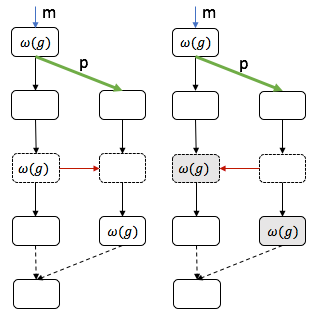
\includegraphics[scale=0.7]{../figs/example-cg}
  \caption{Two computation graphs for the program in \figref{fig:example}: the schedule on the left has no data-race and while the right does.}
%  \vspace{-2em}
   \label{fig:example-cg}
   \end{center}
\end{figure}


\section{Computation Graph and Data-race Detection}
\label{sec:semantics}
A Computation Graph for a task parallel program is a directed acyclic
graph representing the concurrent structure of the program execution
\cite{dennis2012determinacy}.  It is modified here to track memory
locations accessed by tasks.

\begin{definition}
A computation graph is a directed acyclic graph (DAG), $\cg = \tuple{\nodes, \edges, \rv, \wv}$, where $\nodes$ is a finite
set of nodes, $\edges \subseteq \nodes \times \nodes$ is a set of
directed edges, $\rv : (\nodes \mapsto \powerset{\glbls})$ maps $\nodes$ to
the unique identifiers for the shared locations read by the tasks,
$\wv : (\nodes \mapsto \powerset{\glbls})$ maps $\nodes$ to the unique
identifiers for the shared locations written by the tasks, and $\glbls$
is the set of the unique identifiers for the shared locations.
\end{definition}

\algoref{algo:drd} is an algorithm to analyze a computation graph for data-race with
\[
\mathit{conflict}(n_i,n_j) = 
\begin{array}{l}
  \rv(n_i) \cap \wv(n_j) \neq \emptyset\ \vee \\
  \rv(n_j) \cap \wv(n_i) \neq \emptyset\  \vee \\
  \wv(n_i) \cap \wv(n_j) \neq \emptyset\  \\
\end{array}
\]
The notation $n_i \nprec n_j$ means that $n_i$ does not precede $n_j$
in the graph. The complexity of the algorithm is
$|\glbls|*O(|\nodes|^2)$ because computing the transitive closure for
\lineref{loc:path} is $O(|\nodes|*|\edges|)$ and the \textit{conflict}
function is constant.  The algorithm is purposely naive and can be
improved if needed \cite{mellor1991fly,raman2012scalable}.  That said,
problem instances are assumed to be small enough for model checking
which dominates running time since it is limited by the number of
computation graphs that must be enumerated rather than the size of
those graphs.

\begin{algorithm}[t]
  \caption{Data Race detection in a computation graph.} \label{algo:drd}
\begin{algorithmic}[1]
\Function{data\_race}{$\tuple{\nodes, \edges, \rv, \wv}$}
\For {\textbf{each} $n_i,n_j \in \nodes$}
\If {$(n_i \nprec n_j) \wedge (n_j \nprec n_i)$}  \label{loc:path} \label{loc:forall}
   \If {\textit{conflict}$(n_i,n_j,\rv,\wv)$}
      \State {report data-race} \label{loc:datarace}
      \EndIf
\EndIf
 \EndFor
\EndFunction  
\end{algorithmic}
\end{algorithm}


\begin{figure}
  \centering
        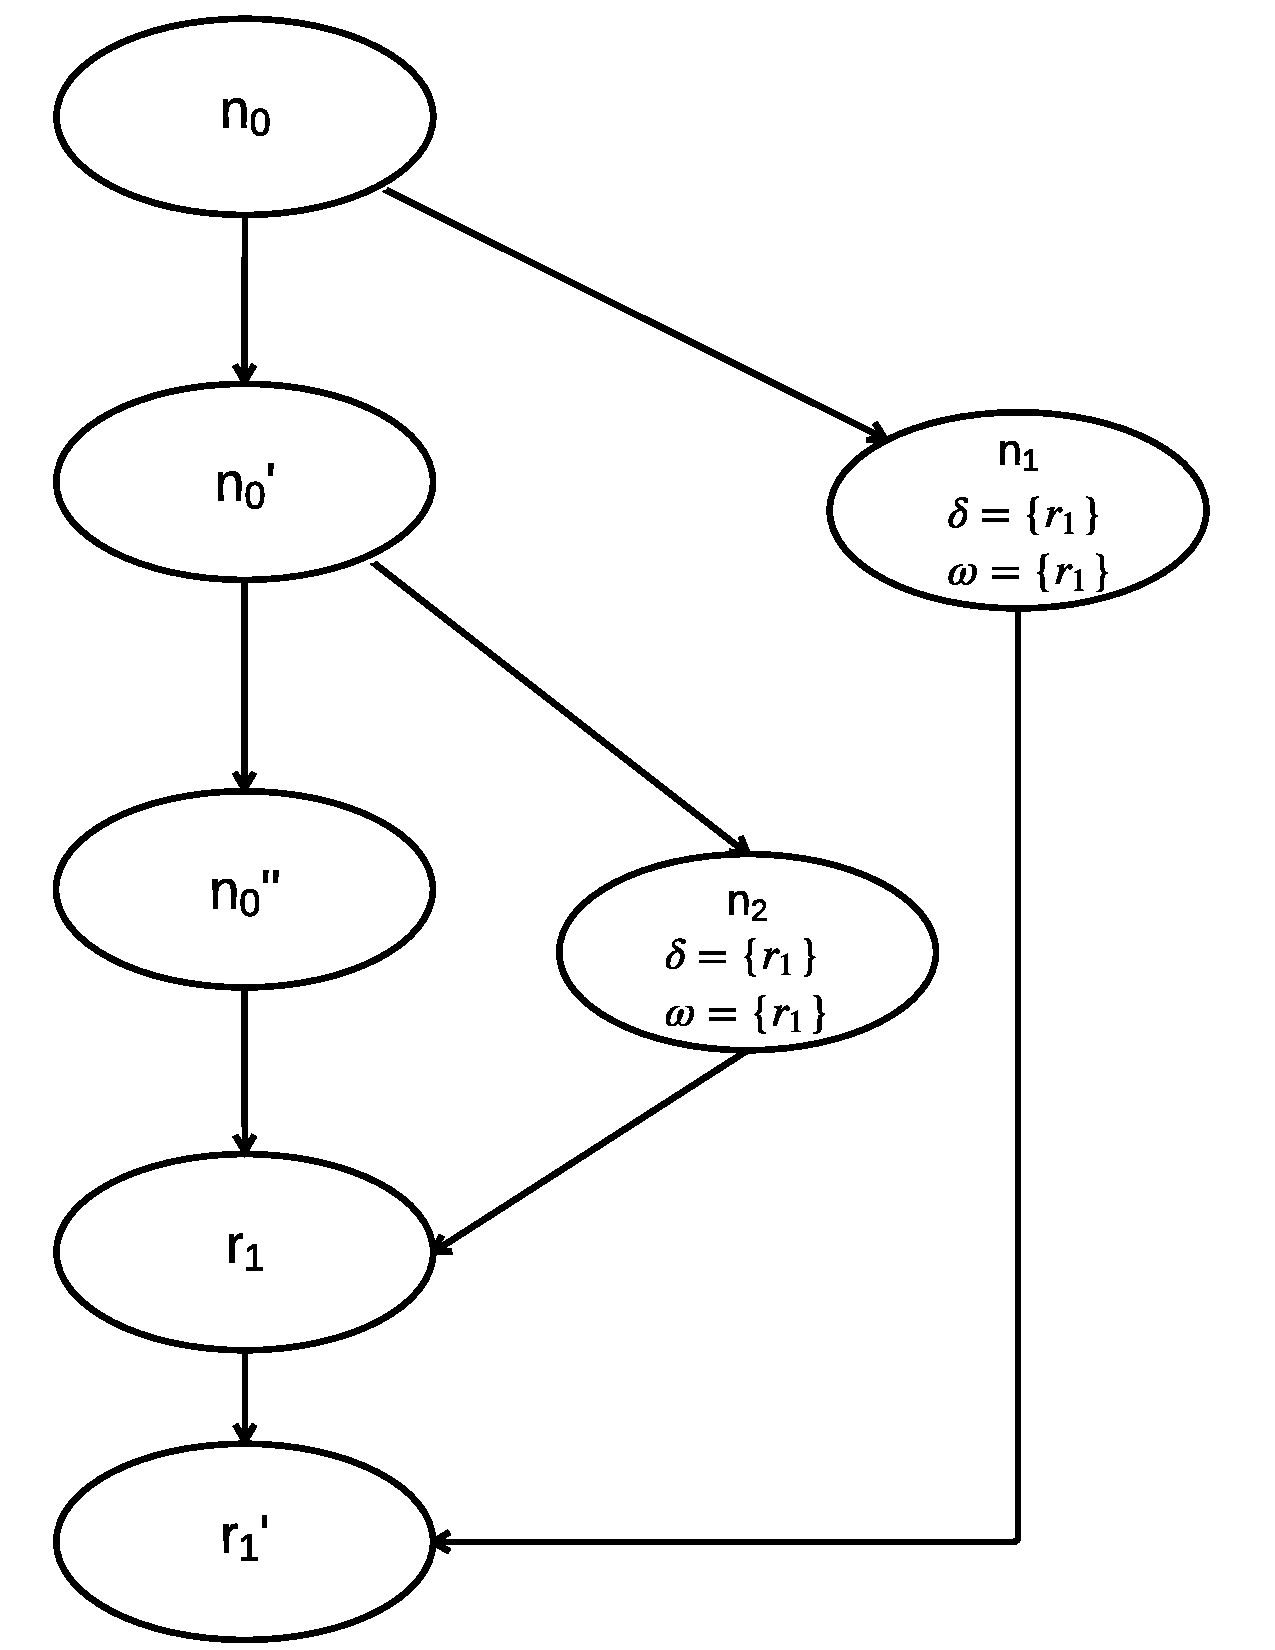
\includegraphics[width=0.3\textwidth]{../figs/Fig3-1.pdf}
    \caption{Computation Graph Example.}
    \label{fig:cg}
    \vspace{-1em}
\end{figure}

\section{Task Parallel Programs} \label{sec:cg}
This section formally defines how to build a computation graph from an
execution trace of a task parallel program.  The programming model is
derived from Bouajjani and Emmi for isolated parallel tasks
\cite{bouajjani}; this variant removes the isolation between tasks
with the introduction of shared memory. It additionally restricts task
passing to only allow tasks to be passed when a child completes, and
those tasks are only passed to the parent.

\subsection{Syntax}
The surface syntax for the language is given in \figref{fig:syntax}.
A program \textbf{P} is a sequence of procedures.  The procedure name
$p$ is taken from a finite set of names \texttt{Proc}.  Each procedure
has a single $L$-type parameter \texttt{l} taken from a finite set of
parameter names \texttt{Vars}; restricting to a single-parameter simplifies the presentation and has no bearing on results.  The
semantics is abstracted over concrete values and operations, so the
possible types of \texttt{l} are not specified. Procedures may also
reference shared variables taking from a finite set of names, $\glbls$,
where $\glbls \cap \mathtt{Vars} = \emptyset$. The names include a
special reserved variable \texttt{isolate} that is only used by the
semantics for mutual exclusion.

The body of a procedure is inductively defined by \textbf{s}.  The
expression language, $e$, is also abstracted and not specified, but
assume it includes variables, references, and a finite set of values
,\texttt{Vals}, that include at least Boolean values.  The set of all
expressions is given by \texttt{Exprs}.

\begin{figure}
  \begin{center}
\[
  \begin{array}{rcl}
\textbf{P} &::=& (\textbf{proc}~p~(\textbf{var}\ \texttt{l} : L)~s)* \\
\textbf{s} &::=& s;~s \alt \texttt{l} := e \alt \textbf{skip} \alt [ \textbf{if}~e~\textbf{then}~s~\textbf{else}~s ] \\
&\alt& [ \textbf{while}~e~\textbf{do}~s ] \alt \textbf{call}~\texttt{l}\ := p~e \alt \textbf{return}~e \\
&\alt& \post~r \leftarrow p~e~d \alt \await~r \alt \ewait~r \\
&\alt& [ \isolated~s ]
  \end{array}
\]
  \end{center}
  \caption{The surface syntax for task parallel programs.}
  %\vspace{-2em}
  \label{fig:syntax}
\end{figure}

The \post-statement, \await-statement, \ewait-statement, and
\isolated-statement relate to concurrency; the rest of the statements
have their usual sequential meaning.  The \post-statement adds a task
into a region $r$, taken from a finite set of region identifiers,
\texttt{Regs}, by indicating the procedure $p$ for the task with an
expression for the local variable value $e$, and a return value
handler $d$ to run in the context of the parent task.  Let
\texttt{Stmts} be the set of all statements and let $\texttt{Rets}
\subseteq (\texttt{Vals} \rightarrow \texttt{Stmts})$ be the set of
return value handlers.

The \await\ and \ewait\ statements synchronize a task with the
sub-ordinate tasks in the indicated region.  Intuitively, when a task
calls \await\ on region $r$, it is blocked until all the tasks it owns
in $r$ finish execution.  Similarly, when a task issues an
\ewait\ with region $r$, it is blocked until one task it owns in $r$
completes.  A task is termed \emph{completed} when its statement is a
\textbf{return}-statement.

The \isolated-statement provides mutual exclusion relative to other
\isolated-statements.  If $s$ is isolated, then it runs mutually
exclusive to any other statements $s^\prime$ that are also isolated;
however, $s$ does not run mutually exclusive to other non-isolated
statements that may be concurrent with $s$.

In addition to the restrictions created by the syntax, we assume that
all programs adhere to the following additional restriction:
procedures with side-effecting return value handlers must be the only
members of their respective regions. This restriction is common to
task-parallel languages.

\subsection{Tree-based Semantics}

The semantics of task parallel programs is defined over trees of
procedure frames to represent the parallelism in the language rather
than stacks which are inherently sequential.  That means that the
frame of each posted task becomes a child to the parent's frame. The
parent-child relationship is transferred appropriately when a parent
completes without synchronizing with its children.  The evolution of
the program proceeds by a task either taking a sequential step or a
concurrency related step that creates, synchronizes, or orders with
other tasks.  The semantics additional define the construction of the
computation graph that is also part of the program state.

A task $t = \tuple{\ell, s, d, n}$ is a tuple containing the value,
$\ell$, of the procedure local variable \texttt{l}, along with a
statement $s$, a return value handler $d$, and an associated node,
$n$, in the computation graph for this task.

A \emph{tree configuration}, $c = \tuple{t,m}$, is an inductively
defined tree with task-labeled vertexes, $t$, and region labeled edges
given by the \emph{region valuation} function, $m : \texttt{Regs}
\rightarrow \texttt{Configs}$, where \texttt{Configs} is the set of
tree configurations.  For a given vertex $c = \tuple{t,m}$, $m(r)$
returns the collection of sub-trees connected to the $t$-labeled root
by $r$-labeled edges. In this context, $m$ is local to the current
task frame. Let $m_o$ be the initial region valuation such that
$\forall r \in \mathtt{Regs}, m_o(r) = \emptyset$.

Contexts are used to simplify the rules for the semantics. A
\emph{configuration context}, $C$, isolates individual task
transitions in the tree (e.g., $C[\tuple{t,m}] \rightarrow
C[\tuple{t^\prime,m}]$ denotes a transition on a
task). Similarly, a \emph{statement context}, $S$, indicates the next
statement to be executed.  A \emph{task statement context}, $T =
\tuple{\ell, S, d, n}$ is a task with a statement context in place of
a statement, and likewise $T[s]$ indicates that $s$ is the next
statement to be executed in the task. Like configuration contexts,
task statement contexts isolate the statement to be executed (e.g.,
$C[\tuple{T[s_1],m}] \rightarrow C[\tuple{T[s_2],m}]$ denotes a transition that modifies the statement in some way).

The \emph{state} of a task parallel program is $\tuple{\cg, \sigma,
  \tuple{t,m}}$ where $\cg$ is a computation graph, $\sigma:
\glbls \rightarrow \mathtt{Vals}$ is a partial function mapping global
variable names in $\glbls$, and $\tuple{t,m}$ is the configuration context for the root of the tree. 

Let $\llbracket \cdot \rrbracket_e$ be an partial evaluation function
for expressions without any variables. For convenience in the
semantics:
\begin{eqnarray*}
  e(t, \sigma) &=& e(\tuple{\ell, s, d, n}, \sigma) \\
  &=& e(\ell, \sigma) \\
  &=& \llbracket e[\ell / \texttt{l}, \sigma(\mathtt{g}_0) / \mathtt{g}_0, \sigma(\mathtt{g}_1) / \mathtt{g_1}, \ldots]  \rrbracket_e
  \end{eqnarray*}
If $e[\ell / \texttt{l}, \sigma(\mathtt{g}_0) / \mathtt{g}_0,
  \sigma(\mathtt{g}_1) / \mathtt{g_1}, \ldots]$ has any free variables
or other errors, then by definition, \\ $\llbracket e[\ell /
  \texttt{l}, \sigma(\mathtt{g}_0) / \mathtt{g}_0,
  \sigma(\mathtt{g}_1) / \mathtt{g_1}, \ldots] \rrbracket_e$ has no
meaning and is undefined. The function is naturally extended to used
contexts as indicated by $e(T)$.  Finally, let the set of shared
variables that appear in $e$ be denoted by $\eta(e,\sigma)$.

As indicated previously, a task $t$ is completed when its next to be
executed statement $s$ is \textbf{return} $e$. Its return-value
handler statement is $\mathrm{rvh}(t) = d(e(T))$ given the task's
context.  By definition, $\mathrm{rvh}(t)$ undefined when $t$ is not
completed or $e(T)$ is undefined.

Finally, the notation, $\rho^\prime = \rho[n \bowtie \eta(e,\sigma)]$
with $\bowtie \in \{\mapstou,\mapsto\}$, indicates the $\rho^\prime$
is just like $\rho$ only if $\bowtie = \mapstou$, then $\rho^\prime(n)
= \rho(n) \cup \eta(e,\sigma)$, and if $\bowtie = \mapsto$, then
$\rho^\prime(n) = \eta(e,\sigma)$. The notation, $m_1^\prime = m
\setminus (r \mapsto \tuple{t_2,m_2})$ means that $m_1^\prime$ is just
like $m$ only $m(r)$ does not include $\tuple{t_2,m_2}$.

The semantics produce a computation graph as a by-product of reducing
the program. Two additional data are associated with the computation
graph and are used by the semantics in the construction: $\last$ is a
special node used to assert the observed order of \isolated-statements
and $\regnodemap : \mathtt{Regs} \mapsto \powerset{\nodes}$ is a function used
to join tasks in a region at synchronization.  In general, a function
notation is adopted to access members of tuples. For example, the
members of the $cg = \tuple{\nodes,\edges, \rv,\wv,\last,\regnodemap}$ are accessed as $\nodes(\cg)$, $\edges(\cg)$,
$\rv(\cg)$, etc.


\begin{figure}
  \begin{center}
    \mprset{flushleft}
    \begin{mathpar}
      \inferrule[Post]
                {
                  n_0^\prime = \mathrm{fresh}() \\
                  n_1 = \mathrm{fresh}() \\
                  \nodes(\cg^\prime) = \nodes(\cg) \cup \{n_0^\prime, n_1\} \\
                  \edges(\cg^\prime) = \edges(\cg) \cup \{\tuple{n_0, n_0^\prime}, \tuple{n_0, n_1}\}\\
                  \rv(\cg^\prime) = \rv(\cg)[n_0 \mapstou \eta(e,\sigma)]\\\\
                  \ell = e(\ell^\prime,\sigma) \\
                  m^\prime = m[r \mapstou \tuple{\tuple{\ell, s_p, d,n_1},m_o}]
                }
                {
                  \tuple{\cg,\sigma,C[\tuple{\ell^\prime,
                        S[\post~r \leftarrow p~e~d],d^\prime, n_0}, m]} \rightarrow \\
                  \tuple{\cg^\prime,\sigma,C[\tuple{\ell^\prime,
                        S[\textbf{skip}],d^\prime, n_0^\prime}, m^\prime]}
                }
      \and
      \inferrule[Await]
                {
                  \regnodemap(\cg^\prime) = \regnodemap(\cg)[r \mapstou \node(t_2)] \\
                  \rv(\cg^\prime) = \rv(\cg)[\node(t_2) \mapstou \eta(e,\sigma)]\\
                  m_1 = m \setminus (r \mapsto \tuple{t_2,m_2}) \\
                  (m_1 \cup m_2)(r) \neq \emptyset \\
                  s(t_2) = \mathbf{return}\ e \\
                  s = d(e(t_2, \sigma))
                }
                {
                  \tuple{\cg,\sigma,C[\tuple{\ell,
                        S[\await~r],d, \node}, m]} \rightarrow \\
                  \tuple{\cg^\prime, \sigma, C[\tuple{\ell,
                        S[s;~\await~r],d, \node}, m_1 \cup m_2]}
                }
      \and
      \inferrule[Await-done]
                {
                  n^\prime = \mathrm{fresh}() \\
                  \nodes(\cg^\prime) = \nodes(\cg) \cup \{\node^\prime\} \\
                  \edges(\cg^\prime) = \edges(\cg) \cup \{\tuple{\node, \node^\prime},\tuple{\node(t_2), \node^\prime}\} \cup
                  \{\tuple{\node_i,\node^\prime} \mid \node_i \in \regnodemap(\cg)(r)\} \\
                  \regnodemap(\cg^\prime) = \regnodemap(\cg)[r \mapsto \emptyset] \\
                  \rv(\cg^\prime) = \rv(\cg)[\node(t_2) \mapstou \eta(e,\sigma)]\\
                  m_1 = m \setminus (r \mapsto \tuple{t_2,m_2}) \\
                  (m_1 \cup m_2)(r) =
                  \emptyset \\
                  s(t_2) = \mathbf{return}\ e \\
                  s = d(e(t_2, \sigma))
                }
                {
                  \tuple{\cg,\sigma,C[\tuple{\ell,
                        S[\await~r],d, \node}, m]} \rightarrow \\
                  \tuple{\cg^\prime, \sigma, C[\tuple{\ell,
                        S[s],d, \node^\prime}, m_1 \cup m_2]}
                }
      \and
      \inferrule[Isolated]
                {
                  n^\prime = \mathrm{fresh}() \\
                  \nodes(\cg^\prime) = \nodes(\cg) \cup \{n^\prime\} \\
                  \edges(\cg^\prime) = \edges(\cg) \cup \{\tuple{n, n^\prime},  \tuple{\last(\cg),n^\prime}\}\\
   				  \sigma(\mathtt{isolate}) = \falsev \\
                  \sigma^\prime = \sigma[\mathtt{isolate} \mapsto \truev]
                }
                {
                  \tuple{\cg,\sigma,C[\tuple{\ell^\prime,S[\isolated~s],d^\prime, n, 0}, m]} \rightarrow \\
                  \tuple{\cg^\prime, \sigma^\prime, C[\tuple{\ell^\prime,
				        S[s; \textbf{isolated-end}],d^\prime, n^\prime, 1}, m]}
                }
      \and
      \inferrule[Isolated-done]
                {
                  n^\prime = \mathrm{fresh()}\\
                  \last(\cg^\prime) = n \\
                  \nodes(\cg^\prime) = \nodes(\cg) \cup \{n^\prime\} \\
                  \edges(\cg^\prime) = \edges(\cg) \cup \{\tuple{n, n^\prime}\} \\
                  \sigma(\mathtt{isolate}) = \truev \\
                  \sigma^\prime = \sigma[\mathtt{isolate} \mapsto \falsev]
                }
                {
                  \tuple{\cg, \sigma, C[\tuple{\ell^\prime,S[\textbf{isolated-end}],d^\prime, n, 1}, m]} \rightarrow \\
                  \tuple{\cg^\prime, \sigma^\prime, C[\tuple{\ell^\prime,
				   S[\textbf{skip}],d^\prime, n^\prime,0}, m]}
                }
                
\end{mathpar}
  \end{center}
  \caption{The transition rules for the inter-procedural statements, task creation, and task synchronization.}
%    \vspace{-2em}
  \label{fig:inter}
    \label{fig:semantics}
\end{figure}

The semantics is given as a set of transition rules relating states.
\figref{fig:inter} contains a subset of the rules pertinent to the
proof of correctness in the next section. The omitted rules for
intra-procedural statements have their usual definition; additionally, the
inter-procedural statement, $\textbf{call}~\texttt{l}\ := p~e$, is
syntactic sugar for
\[
\post~r_\mathit{call}\leftarrow p~e~\lamdefe{v}{\texttt{l} := v};~
\ewait~r_\mathit{call},
\]
where $r_{call}$ is exclusive to the caller containing no other tasks. The semantics create a computation graph as a byproduct of reducing the program. The computation graph observes rather than determines the execution of the program. 

The \textsc{Post} rule creates a new child task. The rule adds two
fresh nodes $n_0^\prime$ and $n_1$ to the computation graph: node
$n_0^\prime$ represents the statements following \post\ and $n_1$
represents the statements to be executed by the new task. The rule
orders both after the current node for the parent, $n_0$, in the
computation graph.  The read set $\rho$ of node $n_0$ is updated to
include any global variables referenced in the expression,
$\eta\left(e\right)$, for the local parameter value in the new
task. The region mapping $m$ of the parent task is updated to include
the new task with its empty initial region mapping.


The \textsc{Await} rule blocks the execution of the currently
executing task until a task in the indicated region completes.  A new
node to join the two tasks is not created in the computation graph,
nor are the two tasks ordered in the sense of join because the choice
of task $t_2$ in the region is non-deterministic; as such, the
computation graph allows tasks in the region to join in any order
contrary to the observed reduction by the rule. The rule saves the
current node in the graph for $t_2$, $\node(t_2)$, to join later once
the region is empty, and it updates the read set for $t_2$ on the
expression in the \textbf{return}-statement. The rest of the rule
separates out the task from the region, makes sure the region is not
yet empty, and gets the statement for the return value handler. The
new state adds an \textbf{await}-statement after the return value
handler statement since the region is not yet empty, and the region
valuation function in the new state includes any tasks owned by
$t_2$.\footnote{The region valuation $m_2$ may actually include tasks
  posted into $r$ because configurations are local rather than
  global. This locality means that two tasks may post into the same
  region, but neither tasks knows about the tasks posted by the other
  into that region.}


The \textsc{Await-Done} activates when the last task in the region is
joined. It differs from the \textsc{Await} rule in that it
orders all tasks that have joined in the region to happen-before the
new node for the parent in the computation graph, and it does not
insert another \textbf{await}-statement in the new state.

The \textsc{Ewait} and \textsc{Ewait-Done} rules, not shown in the
figure, follow \textsc{Await} and \textsc{Await-Done} respectively
only without the recursive statement when the region is not empty
since it only needs to wait on a single task to complete. The rules
delay the ordering of tasks joined in the region to when the region
becomes empty (i.e., the last task joins) just as done for
\textbf{await}-statements.

If no other isolated statements are running, then the
\textsc{Isolated} rule updates the \texttt{isolated} shared variable
and inserts after the isolated statement $\mathit{s}$ the new
\textbf{isolated-end} keyword. The computation graph gets a new node
to track accesses in the isolated statement with an appropriate edge
from the previous node. A sequencing edge from $\last$ is also added
so the previous isolated statement happens before this new isolated
statement. As a note, $\last$ is initialized to the initial node when
execution starts.

The \textsc{Isolated-End} rule creates a new node in the computation
graph to denote the end of isolation, updates the \texttt{isolated}
shared variable, and it updates $\last$ to properly sequence any
future isolation. \textbf{isolated}-statements are totally ordered in
the computation graph.

The initial task for a program is $t_o = \tuple{\ell, s_o,
  \lamdefe{v}{\mathtt{skip}}, n}$ where $\ell$ is the initial value of
the parameter for the top level procedure $p_o$, $s_o = \post r_0
\leftarrow p_0~\ell~\lamdefe{v}{\mathtt{skip}}; \await~r_0$;
$\await~r_1; \ldots$, and $n$ is a fresh node for the computation
graph (i.e., $n = \mathrm{fresh}()$). The initial state of a program
is given as $\tuple{\cg_o, \sigma_o, \tuple{t_o,m_o}}$ where $\cg_o$
is an initial graph such that $N = \{n\}$, $E = \emptyset$, $\rho(n) =
\emptyset$, and $\omega(n) = \emptyset$; $\sigma_o$ maps all global
variables to an initial default value; and $\forall r \in
\texttt{Regs}, m(r) = \emptyset$.


\section{Proof of correctness}
\label{sec:proof}

For a given program and input, the computation graphs produced by the
tree semantics in Section~\ref{sec:semantics} demonstrate a data race
if and only if a data race is possible for the given program and
input.

\begin{comment}
\begin{definition}\label{def:scheduler}
A scheduler is a program capable of deciding which task to reduce,
given a tree configuration.
\end{definition}
\end{comment}

\begin{definition}[\textit{conflict}]
Two statements conflict if they both access the same shared variable
and at least one of them writes to that variable.
$\rv\left(\statement\right)$ and $\wv\left(\statement\right)$ behave
as expected.
\begin{gather*}
\mathit{conflict}(\statement_i,\statement_j) =
\begin{array}{l}
  \rv(\statement_i) \cap \wv(\statement_j) \neq \emptyset\ \vee \\
  \rv(\statement_j) \cap \wv(\statement_i) \neq \emptyset\ \vee \\
  \wv(\statement_i) \cap \wv(\statement_j) \neq \emptyset\ \\
\end{array}
\end{gather*}
\end{definition}

\begin{definition}[Active statements]
A state \st\ has a set of active statements \activestatements{\st}
that corresponds to the next statement to be reduced in each of the
active tasks in the state.
\end{definition}

\begin{definition}[Concurrency]
Two statements are concurrent if and only if an execution of the
program can result in a state \st\ such that both statements are
active at the same time:

\begin{gather*}
\concurrent{\statement}{\statement'} \bimp \exists \st \left(\st_{0}
\overset{*}{\rightarrow} \st \; \wedge \; \left\{\statement,
\statement'\right\} \subseteq \activestatements{\st}\right) .
\end{gather*}

A state \st\ that satisfies this condition for \statement\ and
\statement' is called a witness state for
\concurrent{\statement}{\statement'}.
\end{definition}

\begin{definition}[Data race]
Two statements $\statement$ and $\statement'$ demonstrate a data race if
and only if they conflict and if they are concurrent:

\begin{align*}
\dr\left(\statement, \statement'\right) =
\concurrent{\statement}{\statement'} \; \wedge
\mathit{conflict}\left(\statement, \statement'\right).
\end{align*}
\end{definition}

Two statements that occur in the same thread of execution cannot be
concurrent, as exactly one statement is active in each active thread
at any point in time. Two statements inside of \isolated-statements
cannot be concurrent; once one has entered its \isolated-statement,
all other threads must block upon reaching an \isolated-statement
until the first thread exits its \isolated-statement.

Before proving the correctness of data races in the computation graph,
it is useful to observe that only nodes that end in a \post-statement
and \isolated-statements can have multiple outgoing edges. In both
cases, the edges go to nodes in different threads of execution.
Similarly, only \isolated-statements and nodes following an \await- or
\ewait-statement (in the parent thread) and following
\textbf{return}-statements (in child threads) have multiple incoming
edges. As with \post\ statements, the edges that converge on a node
come from distinct threads of execution.

\begin{lemma}
\label{lemma:concurrent-to-unordered}
If two statements $\statement \in \node$ and $\statement' \in \node'$
are concurrent, \node\ and \node' are unordered in the computation
graph \cg\ in every witness state \st\ for
\concurrent{\statement}{\statement'}:

\begin{gather*}
\text{Given } \, \statement \in \node \text{ and } \statement' \in
\node', \\
\forall \st \left(\st_{0} \overset{*}{\rightarrow} \st \wedge
\left\{\statement, \statement'\right\} \subseteq
\activestatements{\st} \implies
\unrelated{\node}{\node'}{\prec}{\nprec}\right) .
\end{gather*}
\end{lemma}

\begin{proof}
By inspection of the semantics, outgoing edges are created on active
threads' nodes only on or after each respective node's final
reduction. New nodes are always fresh. As such, the nodes for any two
active statements are unrelated.
\end{proof}

\begin{lemma}
\label{lemma:unordered-to-concurrent}
If two nodes $\node$ and $\node'$ are unordered in a state's
computation graph \cg, every $\statement \in \node$ and $\statement'
\in \node'$ are concurrent:

\begin{gather*}
\text{Given} \, \statement \in \node \text{ and } \statement' \in
\node', \unrelated{\node}{\node'}{\prec}{\nprec} \implies
\concurrent{\statement}{\statement'} .
\end{gather*}
\end{lemma}

\begin{proof}

The two nodes \node\ and \node' are both reachable; otherwise, they
would not have been generated in \cg. Within a node, it is possible to
advance or wait independent of other nodes' behaviors. Accordingly, it
is possible to begin at $\st_{0}$ and advance until \statement\ is
active. Similarly, it is possible to advance until \statement' is
active. What remains to be proven is whether or not it is possible to
reach a state where both \statement\ and \statement' are active; in
other words, if it is possible for some schedule to reach \statement\
in one task and then to reach \statement' in some other task without
advancing the first task any further.

By the construction of \cg, \node\ and \node' must have some least
common ancestor $\node_{A}$ that is also reachable. $\node_{A}$ must
either end in a \post-statement or be an \isolated-statement, as the
reduction rules only allow these two statements to have multiple
outgoing edges. In both cases, the child nodes of $\node_{A}$ must be
in different tasks. Without loss of generality, we say that \task\
either contains \node or is some ancestor of the task that does.
Similarly, we say that \task' either contains \node' or is an ancestor
of the task that does.

We first advance to $\node_{A}$ on some schedule that does not
contradict $\prec$. This is possible because $\node_{A}$, \node, and
\node' were all generated. At this point, execution of \task\ and its
children is independent of \task' and its children because $\node_{A}$
is the least common ancestor of \node\ and \node'; no
\isolated-statements can cause one to block on the other, nodes are
generated fresh and so \post-statements cannot link them, and \await-
and \ewait-statements cannot join them. We advance \task\ and any
relevant children until reaching \node\ and then proceed until
reaching \statement. Then, we advance \task' and any relevant children
until reaching \node' and then proceed until reaching \statement'.

At this point, both \statement\ and \statement' are active, so they
must be concurrent.
\end{proof}

Our proof asserts that the computation graph demonstrates a data race
if and only if such a data race exists. As such, we need not reason
about any behaviors that occur after a data race.

\begin{comment}
\begin{definition}[Schedule]
A schedule is a series of states that starts with the initial state
$\st_{0}$. Each state can be derived from its predecessor in the
schedule:

\begin{gather*}
\tuple{\st_{0}, \st_{1}, \ldots, \st} \text{ where } \st_{0}
\rightarrow \st_{1} \rightarrow \ldots \rightarrow \st .
\end{gather*}
\end{definition}

\begin{definition}[Race-free schedule]
A race-free schedule is a schedule that contains only race-free
reductions.
\end{definition}

Data races occur, in one sense, as an interaction between two
different reductions. However, a single reduction is sufficient to
influence downstream behaviors. It is possible to reason about all
race-free schedules without enumerating them.

\begin{definition}[Race-free state]
A race-free state \rf{\st} is a state in a race-free schedule.
\end{definition}
\end{comment}

\begin{lemma}[Soundness of \textit{conflict} over nodes]
\label{lemma:conflict-sound}
If two nodes conflict, there exists a pair of statements, one from
each node, that conflicts:

\begin{gather*}
\mathit{conflict}\left(\node, \node'\right) \implies \exists
\statement \in \node, \statement' \in \node'
\left(\mathit{conflict}\left(\statement, \statement'\right)\right) .
\end{gather*}
\end{lemma}

\begin{proof}
If two nodes conflict, it is because \rv\ and \wv\ were updated in
some reduction. More specifically, if $\rv\left(\node\right) \ne
\emptyset$, at least one statement $\statement \in \node$ must read a
global variable; the reduction of statements that read a global
variable are the only way that \rv\ updates. The same reasoning
applies to \wv.
\end{proof}

\begin{lemma}[Completeness of \textit{conflict} over nodes]
\label{lemma:conflict-complete}
If two statements conflict, their respective nodes will conflict.

\begin{gather*}
\text{Given } \statement \in \node \wedge \statement' \in \node',
\left(\mathit{conflict}\left(\statement, \statement'\right)\right)
\implies \mathit{conflict}\left(\node, \node'\right) .
\end{gather*}
\end{lemma}

\begin{proof}
If $\statement \in \node$, then \statement\ must have been reduced in
\node. By inspection of the semantic rules, $\rv\left(\node\right)$
and $\wv\left(\node\right)$ must be updated to include \statement\ as
necessary. Accordingly, nodes conflict whenever statements they
include conflict.
\end{proof}

\begin{theorem}[Soundness of computation graph over data races]
If a computation graph reports a data race, there is a data race in
the program on the given input.
\end{theorem}
\begin{proof}
By Lemma~\ref{lemma:unordered-to-concurrent} and
Lemma~\ref{lemma:conflict-sound}.
\end{proof}

\begin{theorem}[Completeness of computation graph over data races]
If there is a data race in the program on the given input, a
computation graph generated by the model checker reports a data race.
\end{theorem}
\begin{proof}
The definition of data race states that the two statements must be
concurrent, which implies that it is possible to reach both of them in
the same execution. As a result, any two statements that conflict and
are both reachable will be members of nodes in some computation graph.
By Lemma~\ref{lemma:conflict-complete}, the computation graph
identifies the conflict.

The model checker ensures that a computation graph exists for every
possible ordering on \isolated-statements. Computation graphs are
strict partial orders on nodes. Imposing an order on isolated edges
takes the form of adding a tuple on two unrelated members of the
strict partial order and calculating its closure to create a second
relation and adding the reverse of the tuple to the original relation
and calculating its transitive closure to create a third. The
properties of strict partial orders guarantee that the second and
third relations are also strict partial orders and that any two
members of the strict partial orders (besides the two in the tuple)
that were unrelated in the original order are unrelated in at least
one of the resulting orders.

As such, at least one of the resulting computation graphs will
correctly identify that two statements belong to unordered
nodes. By Lemma~\ref{lemma:concurrent-to-unordered}, the statements
are concurrent.
\end{proof}

\section{Implementation and Results}
\label{sec:res}

The data race detection technique described in this paper has been implemented for Habanero Java. It uses the verification runtime specifically designed to test HJ programs \cite{anderson2014jpf}. This runtime makes use of JPF to schedule and run the programs. JPF is essentially a fully customizable Java virtual machine. JPF is modified by removing its default scheduling-factory that inserts choices on all thread actions and accesses to shared variables. Instead, a new scheduling factory based on Algorithm \ref{algo:isolated} is employed for scheduling. The computation graphs are stored in a directed acyclic graph \cite{jgrapht}. The computation graphs are exported in the dot file format for convenience and as a way to understand the structure of the program \cite{graphviz}.

The data-race detector is created by implementing the methods in the \textit{PropertyListenerAdapter} to create the computation graph. When the runtime passes an object of the type \textit{Task} to the \texttt{objectCreated} method, the \textsc{Post} rule is invoked that adds a new node to the computation graph. When the \textit{stop-finish} is executed, the \textsc{Await-next} rule is invoked that creates a node in the graph to synchronize the tasks in the finish block. The \texttt{executeInstruction} method is used to track memory locations that are accessed by various tasks by updating the node with the location accessed by the task during the execution of that instruction.

The results for this technique have been compared to two approaches implemented by JPF: \textit{Precise race detector} and \textit{Gradual permission regions} on benchmarks that cover a wide range of functionality in HJ. These two approaches are specifically chosen for comparison since the results generated by these approaches are sound for a given input just like the technique discussed in this paper. The results show a significant improvement in the time required for verification. 

The benchmarks used in this study make use of various HJ constructs for achieving task parallelism. They spawn a wide range of tasks with smaller programs having 3-15 tasks going all the way up to 525 tasks for larger programs. The experiments were run on a machine with an Intel Core i5 processor with 2.6GHz speed and 8GB of RAM.

\begin{table*}
\centering
\caption{Benchmarks of HJ programs: Computation graphs vs Permission Regions vs. PreciseRaceDetector}
\rowcolors{1}{light-gray}{white}
\label{tab:results}
\resizebox{\textwidth}{!}{
\begin{tabular}{|m{3.5cm}|c|c|c|c|c|c|c|c|c|c|c|}
\hiderowcolors
\hline
        &      &       & 
        \multicolumn{3}{c|}{\textbf{\textit{Computation graphs}}} & 
		 \multicolumn{3}{c|}{\textbf{\textit{Gradual permission regions}}} &
		\multicolumn{3}{c|}{\textbf{\textit{Precise race detector}}} \\ \hline
		
\textbf{Test ID }& \textbf{SLOC} & \textbf{Tasks} 
& \textbf{States}  & \textbf{Time}  & \textbf{Error Note }
& \textbf{States}  & \textbf{Time}  & \textbf{Error Note }
& \textbf{States}  & \textbf{Time}  & \textbf{Error Note }     \\ \hline

\showrowcolors

\textit{Primitive Array Race} & 39 & 3 
%& 5 & 00:00 & Race
& 5 & 00:00 & Race
& 5 & 00:00 & Race
& 220 & 00:00 & Race \\ \hline

\textit{Substring Search}  & 83 & 59 
%& 64 & 00:03 & Race
& 64 & 00:03 & Race
& 8 & 00:00 & Race 
& N/A & N/A & N/A \\ \hline

\textit{Reciprocal Array Sum} & 58 & 2
%& 12 & 0:00:16 & Race
& 4 & 00:08 & Race
& 32 & 00:06 & Race
& N/A & N/A & N/A \\ \hline

\textit{Primitive Array No Race} & 29 & 3 
%& 5 & 00:00 & No Race
& 5 & 00:00 & No Race
& 5 & 00:00 & No Race 
& 11,852 & 00:00 & No Race \\ \hline

\textit{Two Dim Arrays }& 30 & 11 
%& 15 & 00:01 & No Race
& 15 & 00:00 & No Race
& 15 & 00:00 & No Race 
& 597 & 00:00 & Race* \\ \hline

\textit{ForAll With Iterable} & 38 & 2
%& 9 & 00:00 & No Race
& 9 & 00:00 & No Race
& 9 & 00:00 & No Race 
& N/A & N/A & N/A \\ \hline

\textit{Integer Counter  Isolated} & 54 & 10
%& 24 & 00:01 & No Race
& 24 & 00:01 & No Race
& 1,013,102 & 05:53 & No Race 
& N/A & N/A & N/A \\ \hline

\textit{Pipeline With Futures} & 69 & 5
%& 34 & 0:00:00 & No Race
& 34 & 00:00 & No Race
& 34 & 00:00 & No Race 
& N/A & N/A & N/A \\ \hline

\textit{Binary Trees }& 80 & 525 
%& 632 & 0:00:05 & No Race
& 630 & 00:25 & No Race
& 632 & 00:03 & No Race 
& N/A & N/A & N/A \\ \hline

\textit{Prime Num Counter} & 51 & 25
%& 776 & 00:01 & No Race
& 776 & 00:01 & No Race
& 3,542,569 & 17:37 & No Race 
& N/A & N/A & N/A \\ \hline

\textit{Prime Num  Counter ForAll}  & 52 & 25
%& 30 & 0:00:02 & Race*
& 30 & 00:02 & No Race
& 18 & 00:01 & No Race
& N/A & N/A & N/A \\ \hline

\textit{Prime Num Counter ForAsync}  & 44 & 11 
%& 653 & 0:00:01 & No Race
& 653 & 00:01 & No Race
& 2,528,064 & 15:44 & No Race 
& N/A & N/A & N/A \\ \hline

\textit{Add}  & 67 & 3 
%& 11 & 0:00:01 & No Race 
& 11 & 00:01 & No Race 
& 62,374 & 00:33 & No Race
& 4930 & 00:03 & Race* \\ \hline

\textit{Scalar Multiply}  & 55 & 3 
%& 15 & 0:00:01 & No Race
& 15 & 00:01 & No Race
& 55,712 & 00:30 & No Race 
& 826 & 00:01 & Race* \\ \hline

\textit{Vector Add} & 50 & 3 
%& 5 & 0:00:01 & No Race
& 5 & 00:00 & No Race
& 17 & 00:00 & No Race 
& 46,394 & 00:19 & No Race \\ \hline

\textit{Clumped Access}  & 30 & 3 
%& 9 & 0:00:07 & No Race
& 5 & 00:03 & No Race
& 15 & 00:00 & No Race 
& N/A & N/A & N/A \\ \hline

\end{tabular}}
\vspace{-1em}
\end{table*}

\tableref{tab:results} presents the results of verification of the HJ benchmarks. The number of states explored by JPF and time required for verification by each method is compared. The tests are run for a maximum of an hour before they are terminated manually. If a test does not finish in the time bound or if it runs out of JVM memory, then it is marked as N/A in the table. The error note column shows the results of verification. The tests that produce erroneous results are marked with an asterisk ($\ast$). 

The \textit{Precise race detector} explores all potential executions of the program in a systematic way. Each execution is a sequence of transitions. Each transition takes the system from one state to another. Each transition consists of a sequence of byte-code instructions. JPF groups byte-code instructions such that an instruction that manipulates a shared variable is the first one of a transition. In every state that JPF visits, the \textit{precise race detector} checks all actions that can be performed next. If this collection of actions contains at least two conflicting accesses to a shared variable, then a data-race on the shared variable is reported. The \textit{precise race detector} inserts choices in the scheduler for all thread actions such as thread creation, synchronizations, locks etc. Therefore, it does not complete execution within the stipulated time or runs out of memory even on smaller programs because of the state space explosion. It also reports race for \textit{Two Dimensional Arrays}, \textit{Scalar multiply} and \textit{Vector Add} benchmarks where no data race actually exists in the program. This error is because in precise race detector, the access on an array object looks like a data race since it is not able to see the difference in the indexes.

\textit{Gradual permission regions} use program annotations to reduce the state space of the program \cite{mercer2015model}. Whenever a shared variable is accessed by multiple tasks in the program, the accesses have to be annotated to inform the data-race detector to create different schedules for these accesses. It is prone to human errors because of the need for manual annotation. If the program is annotated incorrectly, the results of data race detection analysis are no longer sound. \textit{gradual permission regions} works better than \textit{precise race detector}. Compared to \textit{computation graphs} in this paper though it falls behind quickly when there are several regions to annotate. A single execution is all that is needed for the \textit{computation graph analysis} while \textit{permission regions} have to enumerate an exponential number of schedules over the regions. The difference in performance is seen in the \textit{Add}, \textit{Scalar multiply} and \textit{Prime number counter} benchmarks. These benchmarks use shared variables that have to be enclosed within regions which results in a large state space for permission regions. The \textit{Prime number counter} benchmark also has isolated sections and therefore, the state space for \textit{computation graphs} is also large compared to other benchmarks.

We also evaluated our data race detector on some real world benchmarks. The \textit{Crypt-af} and \textit{Crypt-f} benchmarks are implementation of the IDEA encrytion algorithm and \textit{Series-af} and \textit{Series-f} are the Fourier coefficient analysis benchmarks adapted from the JGF suite \cite{bull2000benchmark} using \textbf{async-finish} and \textbf{future} constructs respectively. The \textit{strassen} benchmark is adapted from the  OpenMP version of the program in the Kastors suite \cite{virouleau:hal-01081974}. \tableref{tab:results1} shows the results of this evaluation.

\begin{table*}
\centering
\caption{Evaluation of Computation graphs on real world benchmarks}
\rowcolors{1}{light-gray}{white}
\label{tab:results1}
\begin{tabular}{|c|c|c|c|c|c|}
\hiderowcolors
\hline

\textbf{Test ID }& \textbf{SLOC} & \textbf{Tasks} 
& \textbf{States}  & \textbf{Time}  & \textbf{Error Note }\\ \hline

\showrowcolors

\textit{Crypt-af} & 1010 & 259
& 260 & 00:17 & No Race  \\ \hline

\textit{Crypt-f}  & 1145 & 387 
& 775 & 00:46 & No Race \\ \hline

\textit{Series-af} & 730 & 329
& 750 & 00:36 & No Race \\ \hline

\textit{Series-f} & 830 & 354 
& 630 & 00:51 & No Race\\ \hline

\textit{Strassen} & 560 & 3
& 7 & 00:57 & No Race \\ \hline

\end{tabular}
\vspace{-1em}
\end{table*}
\vspace{-2em}
\section{Discussion}
\label{sec:discussion}

\subsection{Comparison to other languages}

Our analysis operates on a language that is similar to Habanero Java,
which is itself based on X10. Unlike our language, Habanero Java
distinguishes between futures and asynchronous procedures. The effect
is that every wait on a region waits for everything in that region. On
the other hand, Habanero Java allows asynchronous procedures' return
value handlers to have side effects, which can create data races.

Cilk has the same ability to post asynchronous threads and wait on all
of them to terminate with the same nondeterminism in the order that
threads join. In Cilk, return value handlers are called inlets and can
combine with nondeterministic thread joining order to create data
races. Cilk++ and Cilk Plus lack inlets.

Multilisp also includes futures. Its pcall mechanism is equivalent to
posting the evaluation of each argument and then waiting for them to
all return.

It is possible to identify data races in side-effecting return value
handlers by enumerating all possible orderings. However, the number of
orderings is the factorial of the number of return value handlers.

One alternative approach to this problem is the replacement that
Cilk++ and Cilk Plus use; instead of allowing return value handlers at
all, they use associative operations to combine results from their
child tasks. Enforcing such a restriction on return value handlers
instead of eliminating them entirely allows programmers to handle
most tasks naturally with similarly strong results.

Reactive systems, such as ReactJS, keep a collection of tasks to
execute. At the end of the main function, the eventloop keyword is
reached and parallel tasks execute atomically in a nondeterministic
order. Each task may post additional tasks to the work queue. Our
language could model reactive systems directly with a nondeterministic
\post\ statement. Because of the structured nature of the parallelism
in such languages, it is possible to create a computation graph with
the main function preceding each task and with each task running
without order with respect to its peers. Tasks that generate others
(parents) must execute before their children do. However, many
reactive systems are designed to run indefinitely rather than to
terminate, which complicates the application of the computation graph
model.

\subsection{Side effects in return value handlers}
\label{sec:side-effects-rvhs}

Return value handlers execute in the context of the waiting thread.
When a thread waits on a region with multiple tasks, the order in
which they join is nondeterministic. This creates a situation where
nondeterminism occurs within a single thread. As such, it is possible
to introduce data races on thread-local variables if the return value
handlers can create side effects.

Naturally, it is possible to expand the definitions of \rv\ and \wv\
so that they consider all variables and not just shared variables. In
order to distinguish between identically-named variables in different
tasks, \rv\ and \wv\ would need to take the task ID into account. This
extension would make the language and analysis more general but could
make the analysis much slower.

\section{Related Work} \label{sec:rel-work}
Data-race detection in \emph{unstructured thread parallelism}, where there is no defined protocol for creating and joining threads, or accessing shared memory, relies on static analysis to approximate parallelism and memory accesses \cite{schonberg1989fly,choi2001static,kahlon2009static,kulikov2010detecting,vechev2011automatic} and then improves precision with dynamic analysis \cite{lamport1978time,Godefroid,flanagan2009fasttrack,EraserUpgrade,dimitrov2014commutativity}. Other approaches reason about threads individually \cite{xu1997rely,flanagan2003thread,henzinger2003thread,malkis2007precise,gotsman2007thread}, rely on  assertions \cite{burnim2009asserting, burnim2010determin, hong2012testing, yu2012maple, terragni2015recontest, yu2014simrt, leon2015unfolding, kahkonen2015unfolding}, use low-overhead instrumentation \cite{nistor2010instantcheck}, or construct type proofs \cite{abadi2006types}. These approaches  make few assumptions about the parallelism for generality and typically have higher cost for analysis. 

\emph{Structured parallelism} constrains how threads are created and joined and how shared memory is accessed through programming models. For example, a locking protocol leads to static, dynamic, or hybrid lock-set analyses for data-race detection that are typically more efficient than approaches to unstructured parallelism \cite{savage1997eraser,engler2003racerx,locksets-msr,elmas2006goldilocks,naik2006effective,elmas2007goldilocks,voung2007relay,kahlon2010universal}. Locking protocols are not directly applicable to task-parallel programming models that also constrain parallelism but often without explicit locking. 

\begin{comment}
Different types of data race detection techniques have been developed. The static race detectors analyze the source code to detect races. The dynamic ones use information from the actual program executions. Another technique for data race detection is model checking. In this method, a model of the system being analyzed is created and whether this model meets the specifications is exhaustively checked.

Static data race detectors require program instrumentation by the users. They can reason about all possible program runs. The major drawback of these systems is that they produce a large number of false-positives. \cite{engler2003racerx,ESC,abadi2006types,naik2006effective,voung2007relay,choi2001static, vechev2011automatic}. 

Dynamic race detectors use use different techniques to detect data races at runtime. The lock-set based tools track the set of locks held by each task during execution. These sets are then used to determine conflicts over shared memory references \cite{savage1997eraser, EraserUpgrade, elmas2006goldilocks, elmas2007goldilocks}. 

Dimitrov et al. developed a dynamic commutativity race detector \cite{dimitrov2014commutativity}. It uses vector clocks along with a commutativity specification to generate a structural representation of parallel programs that is used to locate races. Dynamic race detectors based on hashing asserts if different runs of a parallel program with same input produce different outputs \cite{nistor2010instantcheck}.

Lamport defined the happens-before relation in parallel programs \cite{lamport1978time}. The happens-before relation defines a partial order among all the operations in all the threads of a parallel program. The happen-before relation has been used in various data race detection techniques \cite{kahlon2009static, kahlon2010universal, flanagan2009fasttrack, mellor1991fly, schonberg1989fly, miller1988mechanism}. This approach has also been applied to task parallel languages such as Cilk and X10 \cite{Feng97efficientdetection, Async-Finish-Race}. Two approaches based on the happens-before relation, discussed in the introduction, have been developed for HJ programs \cite{raman2012scalable, drdForFutures}. 

Model checking systematically explores the entire state space of the programs to detect concurrency issues \cite{kulikov2010detecting, vakkalanka2008implementing, Godefroid}. The major drawback of model checking is the explosion in the state space as the program size increases. This technique has been extended to verify various task parallel languages such as HJ, X10 and Chapel\cite{anderson2014jpf, gligoric2012x10x, zirkel2013automated}. As opposed to model checking, predictive analysis observes only a single program execution and generalizes the verification results to all possible schedules. This approach has been applied to detecting communication deadlocks in MPI programs \cite{forejt2014precise}.

Various methods have been developed to tackle the state explosion problem of model checking. Rely-guarantee reasoning verifies threads individually using assertions about other threads \cite{xu1997rely, popeea2012compositional}. Thread modular analysis relies on a similar technique. It verifies threads individually using an abstraction of steps that may be performed by other threads \cite{flanagan2003thread, malkis2007precise, henzinger2003thread, gotsman2007thread}.

Hybrid race detection systems have been developed that combine various techniques to overcome some of the limitations of these methods. Permission regions use static program instrumentation combined with dynamic analysis to detect races \cite{westbrook2012practical, westbrook2012permission}. Gradual permission regions use a similar program instrumentation along with model checking \cite{mercer2015model}. 

This work makes use of the happens-before relation for dynamic analysis of programs and use model checking to ensure all schedules are considered in programs with mutual exclusion. A lot of different techniques create model of programs from program executions and use the models for verification. SATCheck observes the program execution to build a concrete behavior model of program execution and using a SAT solver, it tries to find other interesting behaviors \cite{demsky2015satcheck}. Coverage driven testing uses program execution to create a model of the thread interleavings and shared memory accesses to identify unexplored thread interleavings \cite{hong2012testing, yu2012maple}. Regression testing tools for concurrent programs use changes in the program model to identify shared memory accesses that might be affected by the code changes and identifying thread interleavings that must be explored to expose regression bugs \cite{terragni2015recontest, yu2014simrt}. Dynamic symbolic execution is combined with unfolding of petri-nets to create minimal test-suites for testing multi-threaded programs \cite{leon2015unfolding, kahkonen2015unfolding}.
\end{comment}

\section{Conclusion} \label{sec:conclusion}
This work presents a sound and complete technique for data race detection in task parallel programs using computation graphs.  The computation graph creation is presented with the formal semantics for task parallel languages. A scheduling algorithm to create all computation graph structures for programs containing mutual exclusion is also presented for use in model checking. The data race detection analysis is implemented for a Java implementation of the Habanero programming model using JPF and evaluated on a host of benchmarks. The results are compared to JPF's precise race detector and a gradual permission regions based extension. The results show that computation graph analysis reduces the time required for verification significantly relative to JPF's standards. 

\begin{comment}
This work can be extended in the following ways:
\begin{itemize}
\item The data race detector based on computation graphs explores just one control flow path that is taken by the program execution based on the input. The listener can be extended to explore other control flow paths by using Symbolic Execution.
\item The computation graphs can be created statically using program instrumentation and analyzed to gain performance improvements.
\end{itemize}
\end{comment}


%% Acknowledgments
\begin{acks}                            %% acks environment is optional
                                        %% contents suppressed with 'anonymous'
  %% Commands \grantsponsor{<sponsorID>}{<name>}{<url>} and
  %% \grantnum[<url>]{<sponsorID>}{<number>} should be used to
  %% acknowledge financial support and will be used by metadata
  %% extraction tools.
  This material is based upon work supported by the
  \grantsponsor{GS100000001}{National Science
    This research is funded by NSF Grant 
    Foundation}{http://dx.doi.org/10.13039/100000001} under Grant
  No.~\grantnum{GS100000001}{1302524}.  Any opinions, findings, and
  conclusions or recommendations expressed in this material are those
  of the author and do not necessarily reflect the views of the
  National Science Foundation.
\end{acks}


%% Bibliography
%\bibliography{bibfile}


%% Appendix
%\appendix
%\section{Appendix}

%Text of appendix \ldots
\bibliography{../bib/paper} 

\end{document}
